\documentclass[draft]{agujournal2018}
\usepackage{apacite}
\usepackage{lineno}
\usepackage{amsmath}
\usepackage{xcolor}
\usepackage{lipsum}

%%%%%%%%%%%%%%%%%%%%%%%%%%%%%%%%%%%%%%%%%%%%%%%%%%%%%%%%%%
\begin{document}
\title{%
  Deformations from Sea-Ice Tracker Data \\
  \large Béatrice Duval}

\section{Introduction}

As the ocean currents and winds apply a force on arctic sea-ice, the ice moves and deforms, which can create linear kinematic features (LKFs). Understanding LKFs and the statistical properties of sea-ice deformations is of interest from a climatological, physical and logistical point of view \textit{(Bouchat and Tremblay, 2020)}. Currently, simulated deformations are compared to observations from the Radarsat Geophysical Processor System (RGPS), which cover 1997 to 2008 only. There exists however a new promising alternative to obtain SAR images: the combined use of Sentinel-1 and RCM satellites. While they provide the possibility of an operational use of SAR data on a daily basis, they also offer a more frequent and wider area coverage of the Arctic in comparison to the RGPS dataset.

This project aims at computing arctic sea-ice deformations from Sentinel-1 and RCM icetracker data through the use of one of the two algorithms provided. These algorithms differ in the type of input they can accept: while the first (method 00) takes as input a list of tracked features with their starting and ending Latitude/Longitude positions, the second (method 01) accepts inputs in a X/Y coordinate system. Because the latter method performs fewer data operations and, contrary to the method 00, takes the curvature of the Earth into consideration, we recommend using the method 01.

This document is organized as follows. It first describes both algorithms, method 00 and 01, in section 2.1 and 2.2, respectively. Then, in section 3 and 4, a description of the project structure is provided and the project configuration arguments are defined. Finally, in section 5, we present the output NETCDF file produced by the algorithm.

\section{Algorithms}
\subsection{Method 00}
This algorithm processes the input Latitude/Longitude data in 3 steps. First, a Delaunay triangulation is performed. These results are then converted from Latitude/Longitude to X/Y coordinates in a local Cartesian coordinate system based on a grid presented below. Finally, deformations are computed. 

\begin{figure}[h]
 \begin{center}
   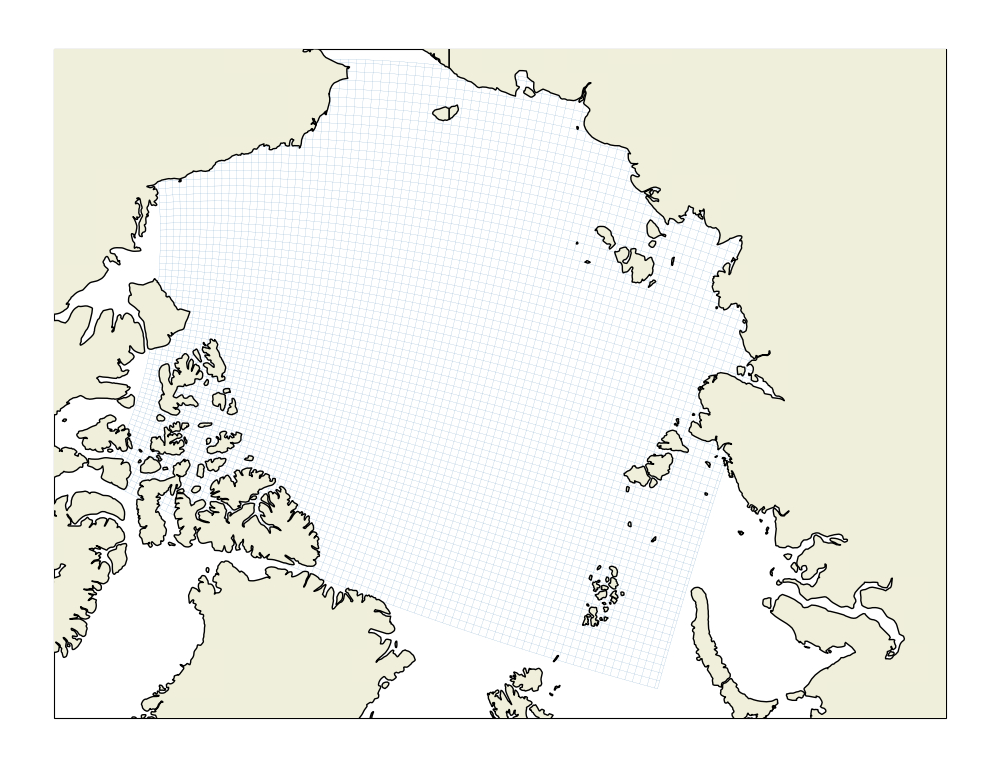
\includegraphics[scale=.4]{figures/grid_lines.png}
 \end{center}
 \caption{A cropped RIOPS grid is used to define the region of interest, as well as to define local Cartesian coordinate systems.}
 \label{grid}
\end{figure}

A grid is used throughout the execution of this algorithm. More specifically, we use a cropped version of the RIOPS grid that defines our region of interest (Fig. \ref{grid}). In addition, the grid stores a distance to land matrix, a land-sea mask, and a matrix of X/Y tracer points. 

The following describes the algorithm in more details.



\subsubsection{Performing a Delaunay Triangulation}

% LIEN VERS LA DOCUMENTATION
First, a Delaunay triangulation algorithm \textit{scipy.spatial.Delaunay} is used to organize the tracked features into triangular arrays. 

\subsubsection{Conversion to Cartesian Coordinates}
\begin{figure}[h]
 \begin{center}
   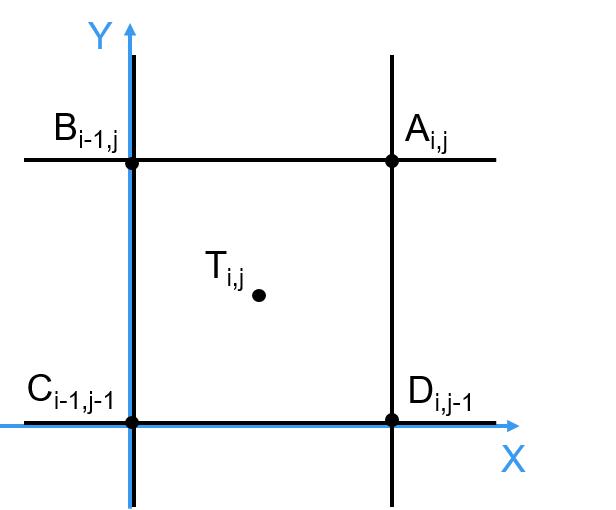
\includegraphics[scale=.6]{figures/localCS.png}
 \end{center}
 \caption{Given a tracer point at (i, j), the origin is defined at the speed point (i-1, j-1), and the x and y-axes are defined by the local grid cell.}
 \label{axes-locaux}
\end{figure}
For every triangle found in the previous step, we want to convert each vertex's starting and ending positions from Latitude/Longitude to X/Y coordinates. In order to avoid conversion errors, we define a local Cartesian coordinate system for each triangle using the RIOPS grid (Fig. \ref{axes-locaux}). That is, for each triangle:

\begin{itemize}
    \item We find the RIOPS grid tracer point nearest to the triangle center (e.g. point T in Fig. \ref{axes-locaux}), and define a ``local cell'' based on the neighbouring speed points (A, B, C and D in Fig. \ref{axes-locaux}).
    % Region of interest: rejection of points is done here
    \item The origin is defined at the Southwest node (C in Fig. \ref{axes-locaux}) and the x and y axis are defined from the southern and eastern cell vertices respectively (sea blue arrows in Fig. \ref{axes-locaux}).
    
    \item Using haversine, we compute the distance between the origin and the nodes B and D, such that we can express their position in the local Cartesian coordinate system: B $ = (0, b)$ and D $=(d,0)$.
\end{itemize}


\begin{figure}[h]
 \begin{center}
   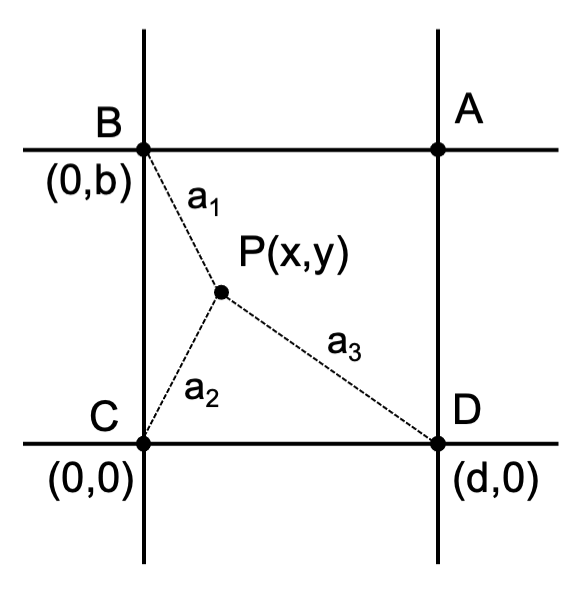
\includegraphics[scale=.6]{figures/triangulation.png}
 \end{center}
 \caption{ We convert the triangle vertex positions from Latitude/Longitude to X/Y coordinates in a local Cartesian coordinate system via triangulation.}
 \label{triangulation}
\end{figure}

We now find the starting and ending positions of each triangle vertex in the local Cartesian coordinate system via triangulation (Fig. \ref{triangulation}):

\begin{itemize}
    
    \item Using haversine, we find the distances $a_1, a_2$ and $a_3$ between the vertex P and the nodes B, C and D. 
    
    \item We now have 3 circles centered at B, C and D and with $a_1, a_2$ and $a_3$ radii, respectively. The X/Y position of the vertex P corresponds to the intersection of the 3 circles. More specifically,
    
\begin{align}
    x = \frac{a_2^2-a_3^2+d^2}{2d} \;\; \text{and} \;\;
    y = \frac{a_2^2-a_1^2+b^2}{2b}.
\end{align}
  
\end{itemize}

\textit{Rejection of Data}

If the distance between a triangle's center point and its nearest grid tracer point is greater than 10 km, we reject that data set since it is not within the region of interest defined by the RIOPS grid (neighboring tracer points are at most 8 km apart). Moreover, we reject a triangle if its tracer point's distance to land is 0, that is if the triangle is located on land. Lastly, once we have the triangle's vertex positions in Cartesian coordinates, we compute its angles and reject it if it has an angle of less than 10 degrees. 

Otherwise, we proceed to the next step, that is computing deformations.



\subsubsection{Computing Deformations}

We compute deformations for every triangle using X/Y coordinates in a local Cartesian coordinate system as computed in the previous step and following \textit{Bouchat et al. (2020)}. The following is taken from \textit{Bouchat et al. (2020)} and presents the equations used to compute deformations.


%%%%%%%%%%%%%%%%%%%%
The total sea-ice deformation rates are defined as:
\begin{equation}
\dot{\epsilon}_{tot} = \left[ \dot{\epsilon}^2_{I}+\dot{\epsilon}^2_{II} \right]^{1/2} \;,
\end{equation}
where 
\begin{eqnarray}
\dot{\epsilon}_{I} &= &\frac{\partial u}{\partial x}+\frac{\partial v}{\partial y} \, , \label{eq:eps_I} \\
\dot{\epsilon}_{II} &= &\left[ \left( \frac{\partial u}{\partial x} - \frac{\partial v}{\partial y}\right)^{2} + \left( \frac{\partial u}{\partial y} + \frac{\partial v}{\partial x}\right)^{2}   \right]^{1/2} \, , \label{eq:eps_II} 
\end{eqnarray}
are the strain rate invariants (or divergence and maximum shear strain rate respectively), and $(u,v)$ are the ice velocity components. In a Lagrangian framework, the velocity derivatives (or strain rates) are most easily obtained using line integrals around the cells contour as per the divergence theorem \textit{(Lindsay, 2003)}: 
\begin{eqnarray}
\frac{\partial u}{\partial x}  = \frac{1}{A}\oint u \textrm{d}y \, ,&  \hspace{0.4cm} & \frac{\partial u}{\partial y}  = -\frac{1}{A}\oint u \textrm{d}x \, , \nonumber \\
\frac{\partial v}{\partial x}  = \frac{1}{A}\oint v \textrm{d}y \, ,&  \hspace{0.4cm}  & \frac{\partial v}{\partial y}  = -\frac{1}{A}\oint v \textrm{d}x\, ,
\label{eq:dudx}
\end{eqnarray}
where A is the Lagrangian cell area. If $(x_{i}, y_{i})$ is the position of the cell vertex $i$ ($=1,2,..,n$; counterclockwise) at time $t$ and $(u_{i}, v_{i})$ its velocity during the time interval $\Delta t_{i}$, we can approximate the line integrals using the trapezoidal rule as:
\begin{equation}
\frac{\partial u}{\partial x}  = \frac{1}{A}\sum_{i=1}^{n}\frac{1}{2}\left( u_{i+1} + u_{i} \right)\left( y_{i+1} - y_{i} \right) \, ,
\label{eq:dudx_sum}
\end{equation}
 where
 \begin{equation}
 A = \frac{1}{2}\sum_{i=1}^{n}\left( x_{i}y_{i+1} -  x_{i+1}y_{i} \right)\, ,
\label{eq:A}
 \end{equation}
and $x_{n+1} = x_1$, and similar other cyclical equalities for $y_{n+1}$, $u_{n+1}$, and $v_{n+1}$. Similar equations also hold for the other velocity derivatives. Here, $(u_{i},v_{i})$ is computed as $(\Delta x_{i}/\Delta t_{i}, \Delta y_{i}/\Delta t_{i})$, where $\Delta x_{i}$ and $\Delta y_{i}$ are the displacement of the cell's vertices during the time interval $\Delta t_{i}$. Note that Equation (\ref{eq:A}) is also derived using the divergence theorem and the trapezoidal rule.
%%%%%%%%%%%%%%%%%%%%%

\subsection{Method 01}

This algorithm processes the input data in X/Y coordinates in 2 steps. A Delaunay triangulation is first performed, and is followed by the computation of deformations. The following describes these steps.

\subsubsection{Performing a Delaunay Triangulation}

The Delaunay triangulation is performed as described in section 2.1.1. We reject triangles that have an angle of less than 10 degrees.

\subsubsection{Computing Deformations}

We compute deformations for every triangle following \textit{Bouchat et al. (2020)} (equations 2 to 7).

\section{Project Structure}

In the following, we describe the structure of the project. We start by presenting the configuration INI file and module in section 3.1. We then present the data processing modules in section 3.2. Finally, we present the visualisation and utility modules in section 3.3 and 3.4, respectively. 


% methods M00 in names

\subsection{Configuration}

The user can configure the project by modifying the definitions of the parameters in namelist.ini. The config module reads these parameters. It then uses them to create a list of data files to process and lists of paths to which data files of all stages of data processing are to be written and loaded. The config module is imported by all data processing modules in order to retrieve configuration parameters, as well as the lists of input and output data file paths.

The following provides a more detailed description of namelist.ini and config.

\begin{description}

  \item[namelist.ini -- ]  Configuration file that contains configuration parameter definitions (see section 4 for further details).
    
    \item[config --] Configuration module that first retrieves configuration arguments from namelist.ini. From a folder (specified in namelist.ini), it then selects raw datasets that satisfy time requirements specified in namelist.ini. That is, datasets that start at a specific date and have a specific duration (± 6 hours) are selected for data processing. From that selection process, a list of raw datasets to process is created, and from that list, lists of paths to which data files of all stages of data processing are to be written and loaded are created.
\end{description}

\subsection{Data Processing}

In order to launch a data processing experience, the main module must be executed. Depending on the method specified in namelist.ini (method 00 or 01), the main module executes in chain the main functions from the appropriate data processing modules. That is, if we are using the method 00, the main module will use processing modules in the following order: M00\_d01\_delaunay\_triangulation, M00\_d02\_to\_grid\_coord\_system and M00\_d03\_compute\_deformations. If we are using the method 01, the order will be: M01\_d01\_delaunay\_triangulation and M01\_d03\_compute\_deformations. If the visualise parameter in namelist.ini is set to `yes', the main function of the visualise\_deformation module is called in order to visualise the output.

In the following, the data processing modules are presented in more details.

\subsubsection{Main Module}

\begin{description}
    \item[main -- ]
    Module that performs all steps of data processing using the method specified in namelist.ini and by calling the main functions of the triangulation, conversion (for method 00 only) and calculations modules described below. If the visualise parameter in namelist.ini is set to `yes', it calls the main function of the visualise\_deformation module described below.
\end{description}

\subsubsection{Method 00 Modules}

The modules listed below follow the method 00 as described in section 2.1.

\begin{description}
  \item[M00\_d00\_crop\_grid --]
    Module that creates a modified RIOPS grid. This module is not imported by the main module and should be executed only once to produce a grid. It takes as input the RIOPS grid and its bathymetry data, and produces a cropped grid in NETCDF4 format (all for which the path is specified in namelist.ini). The output grid stores tracer points (in Latitude/Longitude and X/Y coordinates in the Azimuthal Equidistant projection), speed points (in Latitude/Longitude coordinates), distances between tracer points and land (in km), and a sea-land mask.

  \item[M00\_d01\_delaunay\_triangulation --]
    Module that performs a Delaunay triangulation for all raw DAT files listed in config. It then stores the results in a triangulated CSV file for each dataset, using the triangulated data paths listed in config.

  \item[M00\_d02\_to\_grid\_coord\_system --] Module that converts triangle vertices' starting and ending positions from Latitude/Longitude to X/Y coordinates in a local Cartesian grid coordinate system, for all triangulated CSV files listed in config. It then stores the results in a converted CSV file for each dataset, using the conversion data paths listed in config.

   \item[M00\_d03\_compute\_deformations --]
    Module that computes sea-ice deformations for triangle cells for all converted CSV files listed in config. The results are then stored in a calculations CSV file for each dataset, using the calculations data paths listed in config.
\end{description}

\subsubsection{Method 01 Modules}
The modules listed below follow the method 01 as described in section 2.2.
\begin{description}
   \item[M01\_d01\_delaunay\_triangulation --] Module that performs a Delaunay triangulation on a set of X/Y data points for all raw DAT files listed in config. The results are stored in a triangulated CSV file for each dataset, using the triangulated data paths listed in config.

   \item[M01\_d03\_compute\_deformations --]
    Module that computes sea-ice deformations for triangle cells for all triangulated CSV files listed in config. The results are then stored in a calculations CSV file for each dataset, in addition to a single output NETCDF4 file that combines the results from all processed datasets, using the calculations and output data paths listed in config.
    
\end{description}

\subsection{Visualisation}

In the following, we present the output visualisation module. 

\begin{description}
    
    \item[visualise\_deformation --] Module that plots total sea-ice deformations, divergence, rotation and shear strain rates for all datasets listed in config. 

\end{description}

\subsection{Utility Modules}

The utility modules listed in the following are used in all configuration and processing modules. Here, we describe their general purpose.

\begin{description}
   
    \item[utils\_datetime --] Module that provides tools for finding the starting and ending times of a dataset as Datetime objects given its filename, and for finding the time lapse in seconds between two Datetime objects.
    
    \item[utils\_deformation\_computations --] Module that provides tools for the calculation of sea-ice deformations.      
    
    \item[utils\_get\_data\_paths --]  Module that provides tools that produce data file paths for each stage of data processing given a raw filename, an output folder, an experience name, a starting date and a duration (all of which are parameters in namelist.ini). These data file paths are used to write and load data files from all stages of data processing.
    
    \item[utils\_grid\_coord\_system --] Module that provides tools for the conversion of a triangle's starting and ending positions from Latitude/Longitude to X/Y coordinates in a local Cartesian grid coordinate system.
    
    \item[utils\_load\_data --] Module that provides tools for loading files from all stages of data processing. 
    
    \item[utils\_load\_grid --] Module that provides a tool for loading the project grid.

    
\end{description}


\begin{description}
  \item[]
    
\end{description}

\section{Parameters}

In the following, we define configuration arguments listed in namelist.ini.

\subsection{Input/Output}

The input/output (IO) parameters that follow define the path of the input and output files.

\begin{description}
\item[data\_folder --] Absolute path of the folder from which datasets are selected for processing.

\item[output\_folder --] Absolute path of the folder in which the algorithm's outputs are stored. Outputs from all experiences will be stored under output\_folder.

\item[exp --] Name of the current experience. Outputs of the current experience will be stored under output\_folder/exp.
\end{description}

\subsection{Grid}

The grid parameters below are strictly used in method 00. 

\begin{description}
\item[riops\_grid --] Absolute path of the netcdf file that stores the original RIOPS grid (used in M00\_d00\_crop\_grid module).

\item[bathymetry --]  Absolute path of the netcdf file that stores a bathymetry dataset (used in M00\_d00\_crop\_grid module).

\item[cropped\_grid --] Absolute path of the netcdf file that stores the cropped RIOPS grid (created in M00\_d00\_crop\_grid module).

\end{description}

\subsection{Metadata}

The metadata parameters that follow are used in the creation of NETCDF4 file outputs.

\begin{description}

\item[ice\_tracker --] (S1/RCM) Sea-ice motion tracker.
 
\item[tracking\_error --] Resolution or tracking error (meters) of the sea-ice motion tracker.

\end{description}

\subsection{Processing Options}

The processing options parameters that follow control the way by which datasets are processed.

\begin{description}

\item[overwrite --] (yes/no) When the overwrite argument is set to `yes', all raw data sets that have  already been processed will be re-processed and the resulting CSV files for all stages of data processing will be overwritten. Otherwise, raw data sets that have already been processed will not be re-processed. In any case, an output NETCDF4 file is written with all datasets listed in config for which the deformation calculations could be performed.

\item[method --]  (M00/M01) Method to be used when processing datasets.

\item[visualise --] (yes/no) When the visualise argument is set to `yes', the main function from the visualise\_deformation module is executed by the main module. That is, plots of total sea-ice deformations, divergence and shear strain rates are created and saved under output\_folder/exp/figs. These plots combine output data from all processed datasets.

\end{description}



\subsection{Date Options}

The date options that follow define the time requirements used to select datasets for processing.

\begin{description}
\item[start\_year --]  (YYYY) Starting year of the datasets to process.

\item[start\_month --] (MM) Starting month of the datasets to process.

\item[start\_day --]  (DD) Starting day of the datasets to process.

\item[duration --]   Time span (days) of the datasets to process.
\end{description}

\section{Output NETCDF File}

The method 01 algorithm produces a NETCDF4 file at the end of its execution. This output file combines all datasets that have a common start date and time interval (± 6 hours). On one hand, it stores metadata, which includes the tracking error (or resolution), the satellite which captured the SAR images from which the ice-tracker data was produced (all of which can be specified in the metadata section of namelist.ini), and a reference time. The latter reference time corresponds to the common starting date of the datasets at time 00:00:00. On the other hand, it stores arrays of data organized by triangle: the starting and ending times (in seconds since the reference time), the starting and ending Lat/Lon positions of each vertex, the divergence and the shear ($days^{-1}$).

\end{document}